\chapter{Appendix: Rapid Spanning Tree and White Rabbit}
\label{appD}

\section{Rapid Spanning Tree}

The end goal of STP is to ensure that only one port of a switch is responsible 
for forwarding traffic from the direction of the Root Switch onto any given
link. In networks running STP, every bridge has a priority value associated with
it, according with this value, the switch with the lowest priority will become
the Root of the network.  This process is done by the exchange of BPDUs packets
(Bridge Protocol Data Units) between switches. The rest of the switches shall be
Designated Switched, which forwards packets from the LAN toward the root bridge,
and vice versa.

\begin{center}
        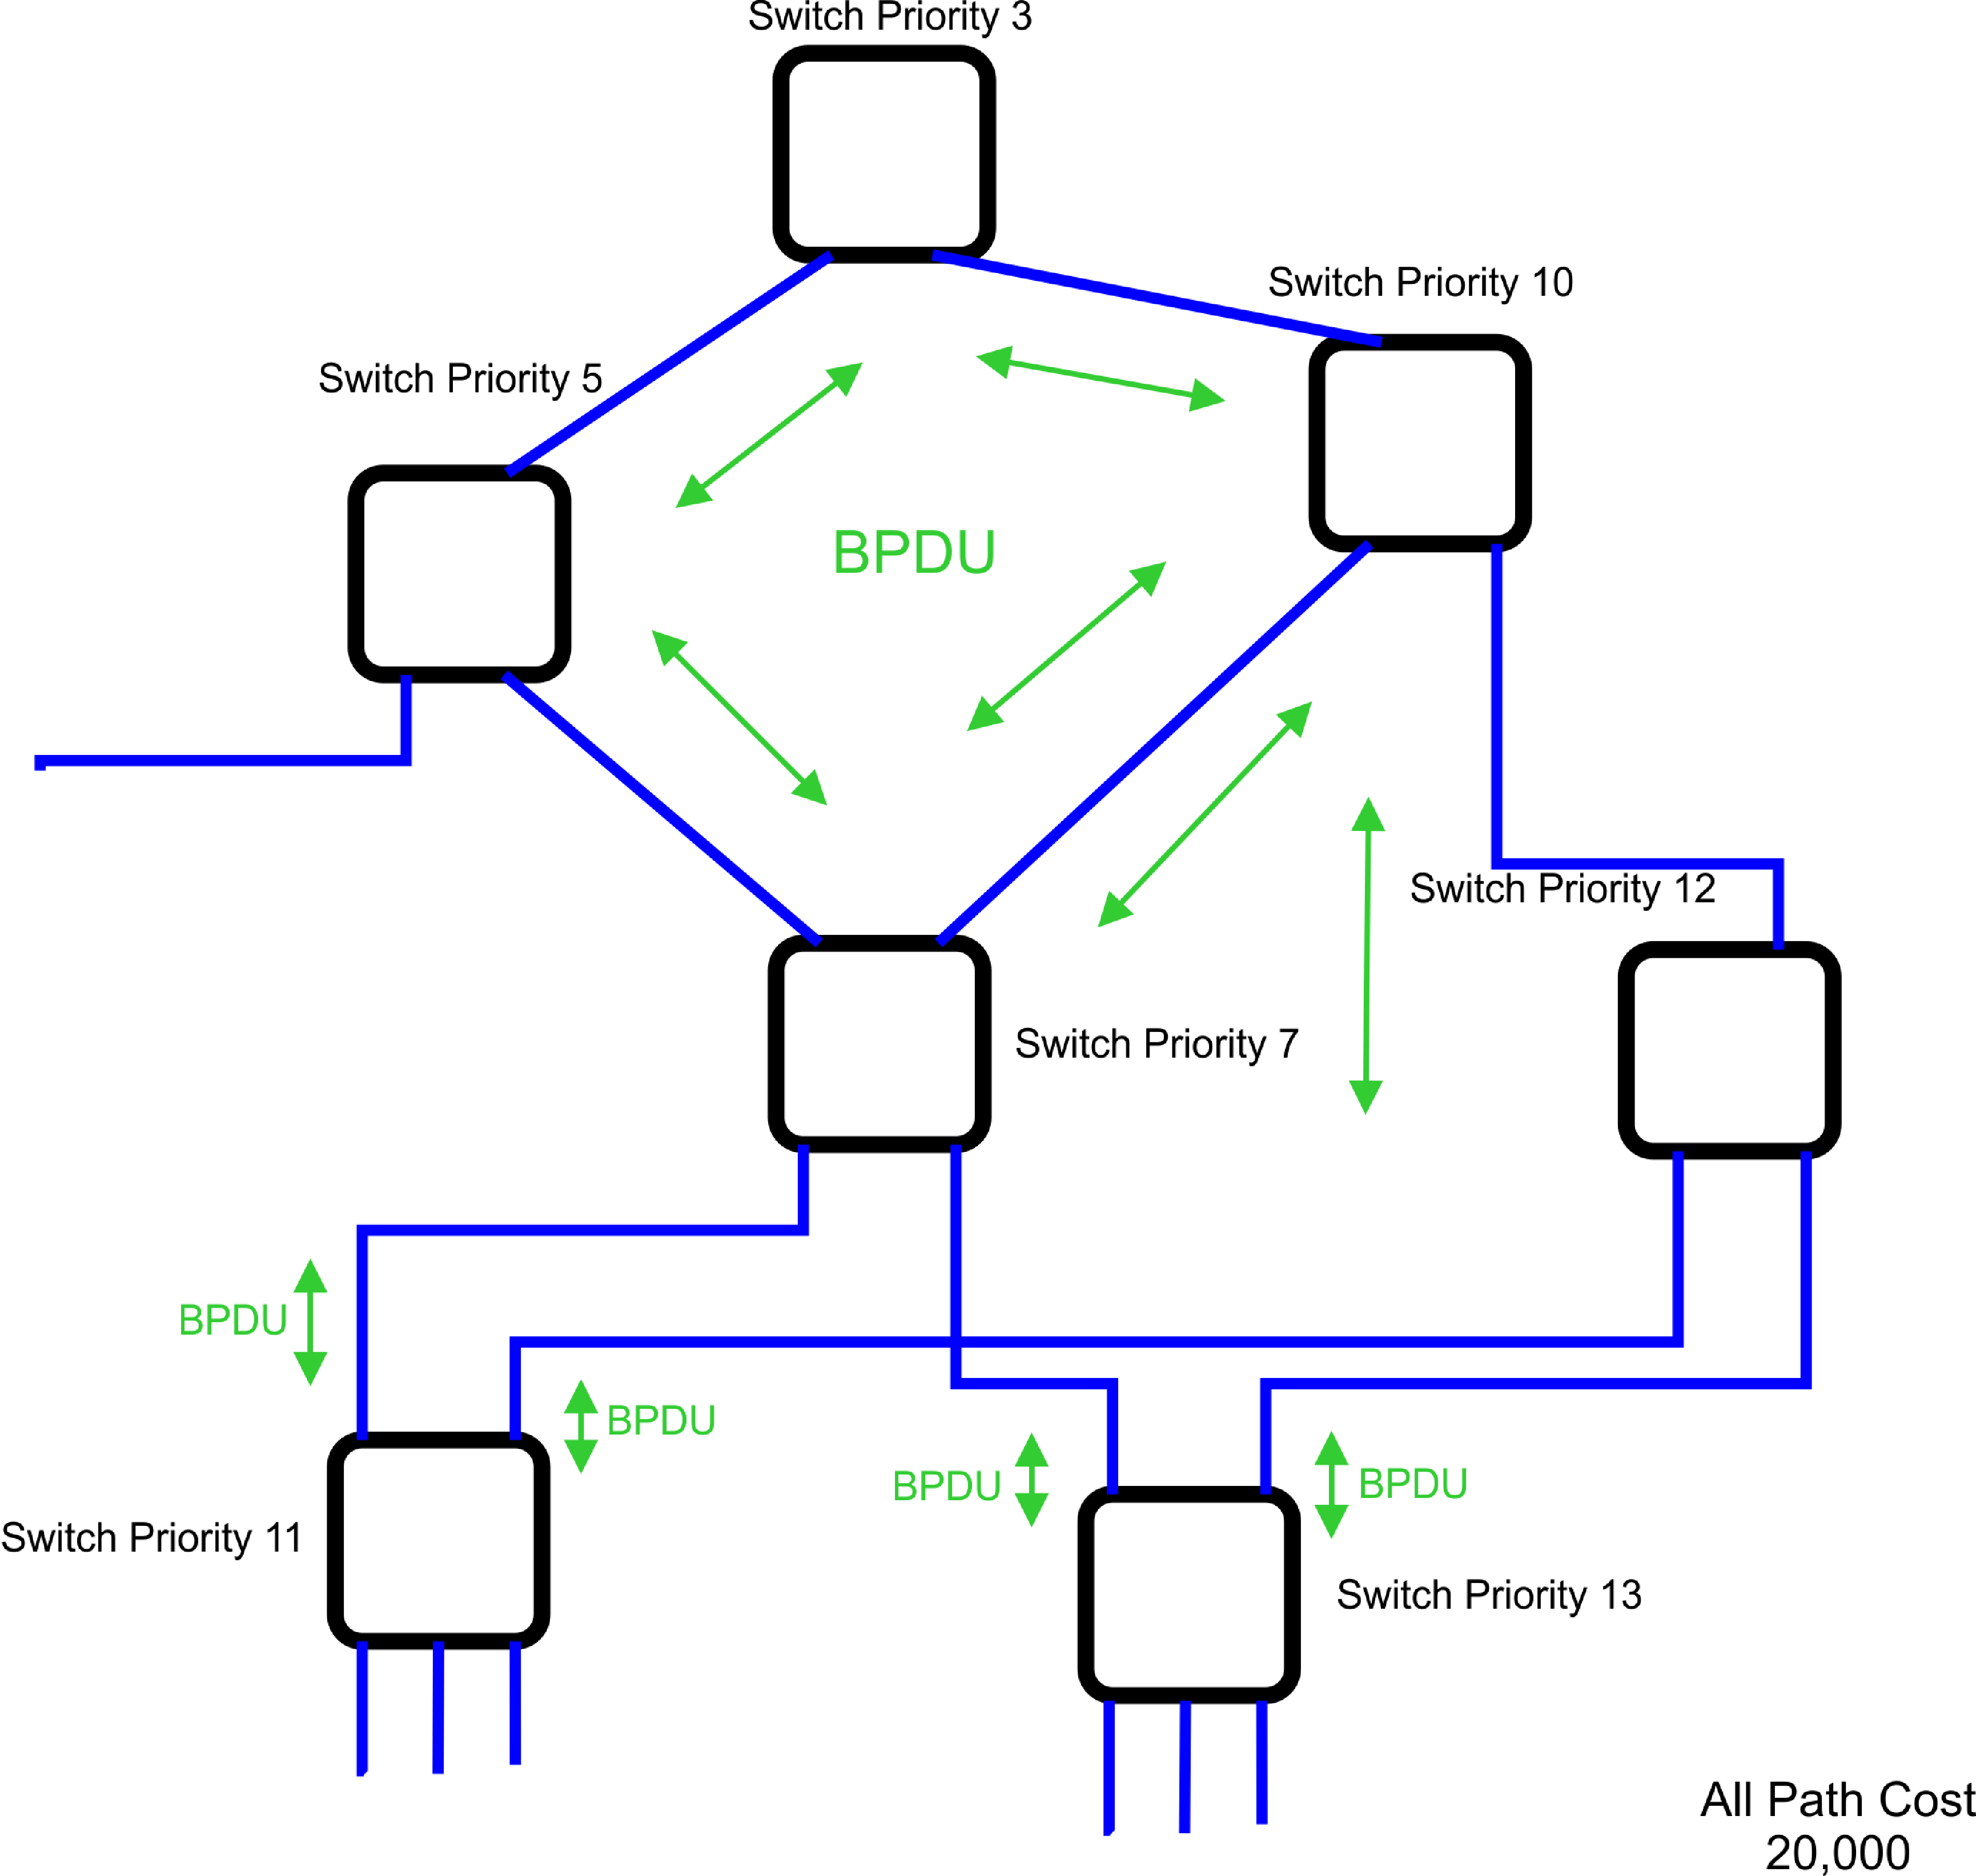
\includegraphics[scale=0.20 ]{robustness/network_beginning.pdf}
        \captionof{figure}{Redundant Network with Loops}
        \label{fig:redunt_net}
\end{center}


Once that the Root Switch has been defined, the switches shall determine
the least cost paths to the Root Switch. The cost is based on the number of
links from the switch till the root, and the cost of every link is based on the
Data Rate of the link. Data Rate ref(table of "Data rate and STP path cost"). In
case that two path have the same cost, there is a mechanism for breaking the
tie.

\begin{itemize}
        \item Root Port: provides connectivity to the root bridge
        \item Designated Port: forwards traffic from the root port onto the
next link.
        \item Alternate Port: an alternate path to the root bridge.
        \item Backup Port: a backup/redundant link to a segment where
another bridge port already connects.
\end{itemize}


RSTP implements distributed variation of Bellman-Ford iterative
algorithm, which could be described as "gradient" process, meaning it iteratively looks for the
optimal solution, selecting an "optimal" candidate every time. Every switch
(with except to the root) send and  accepts BPDU packets
with its information. The switch retains only the best current Root Switch
information electing one root port upstream toward the root switch. The switch
then block alternate paths to the root switch, leaving only the single optimal
upstream path and continue relaying optimal information downstream. If a switch
learns of a better root switch, on any of its ports, the previous "best"
information is erased and the new one immediately accepted and relayed. This
proccess will be propagated to all the switches, and it leads to the convergence
of the network where only one switch will be identified as root, and the rest of
the switches as designated with one port as Root Port and the rest Designated,
Alternate or Backup Port.


\begin{center}
        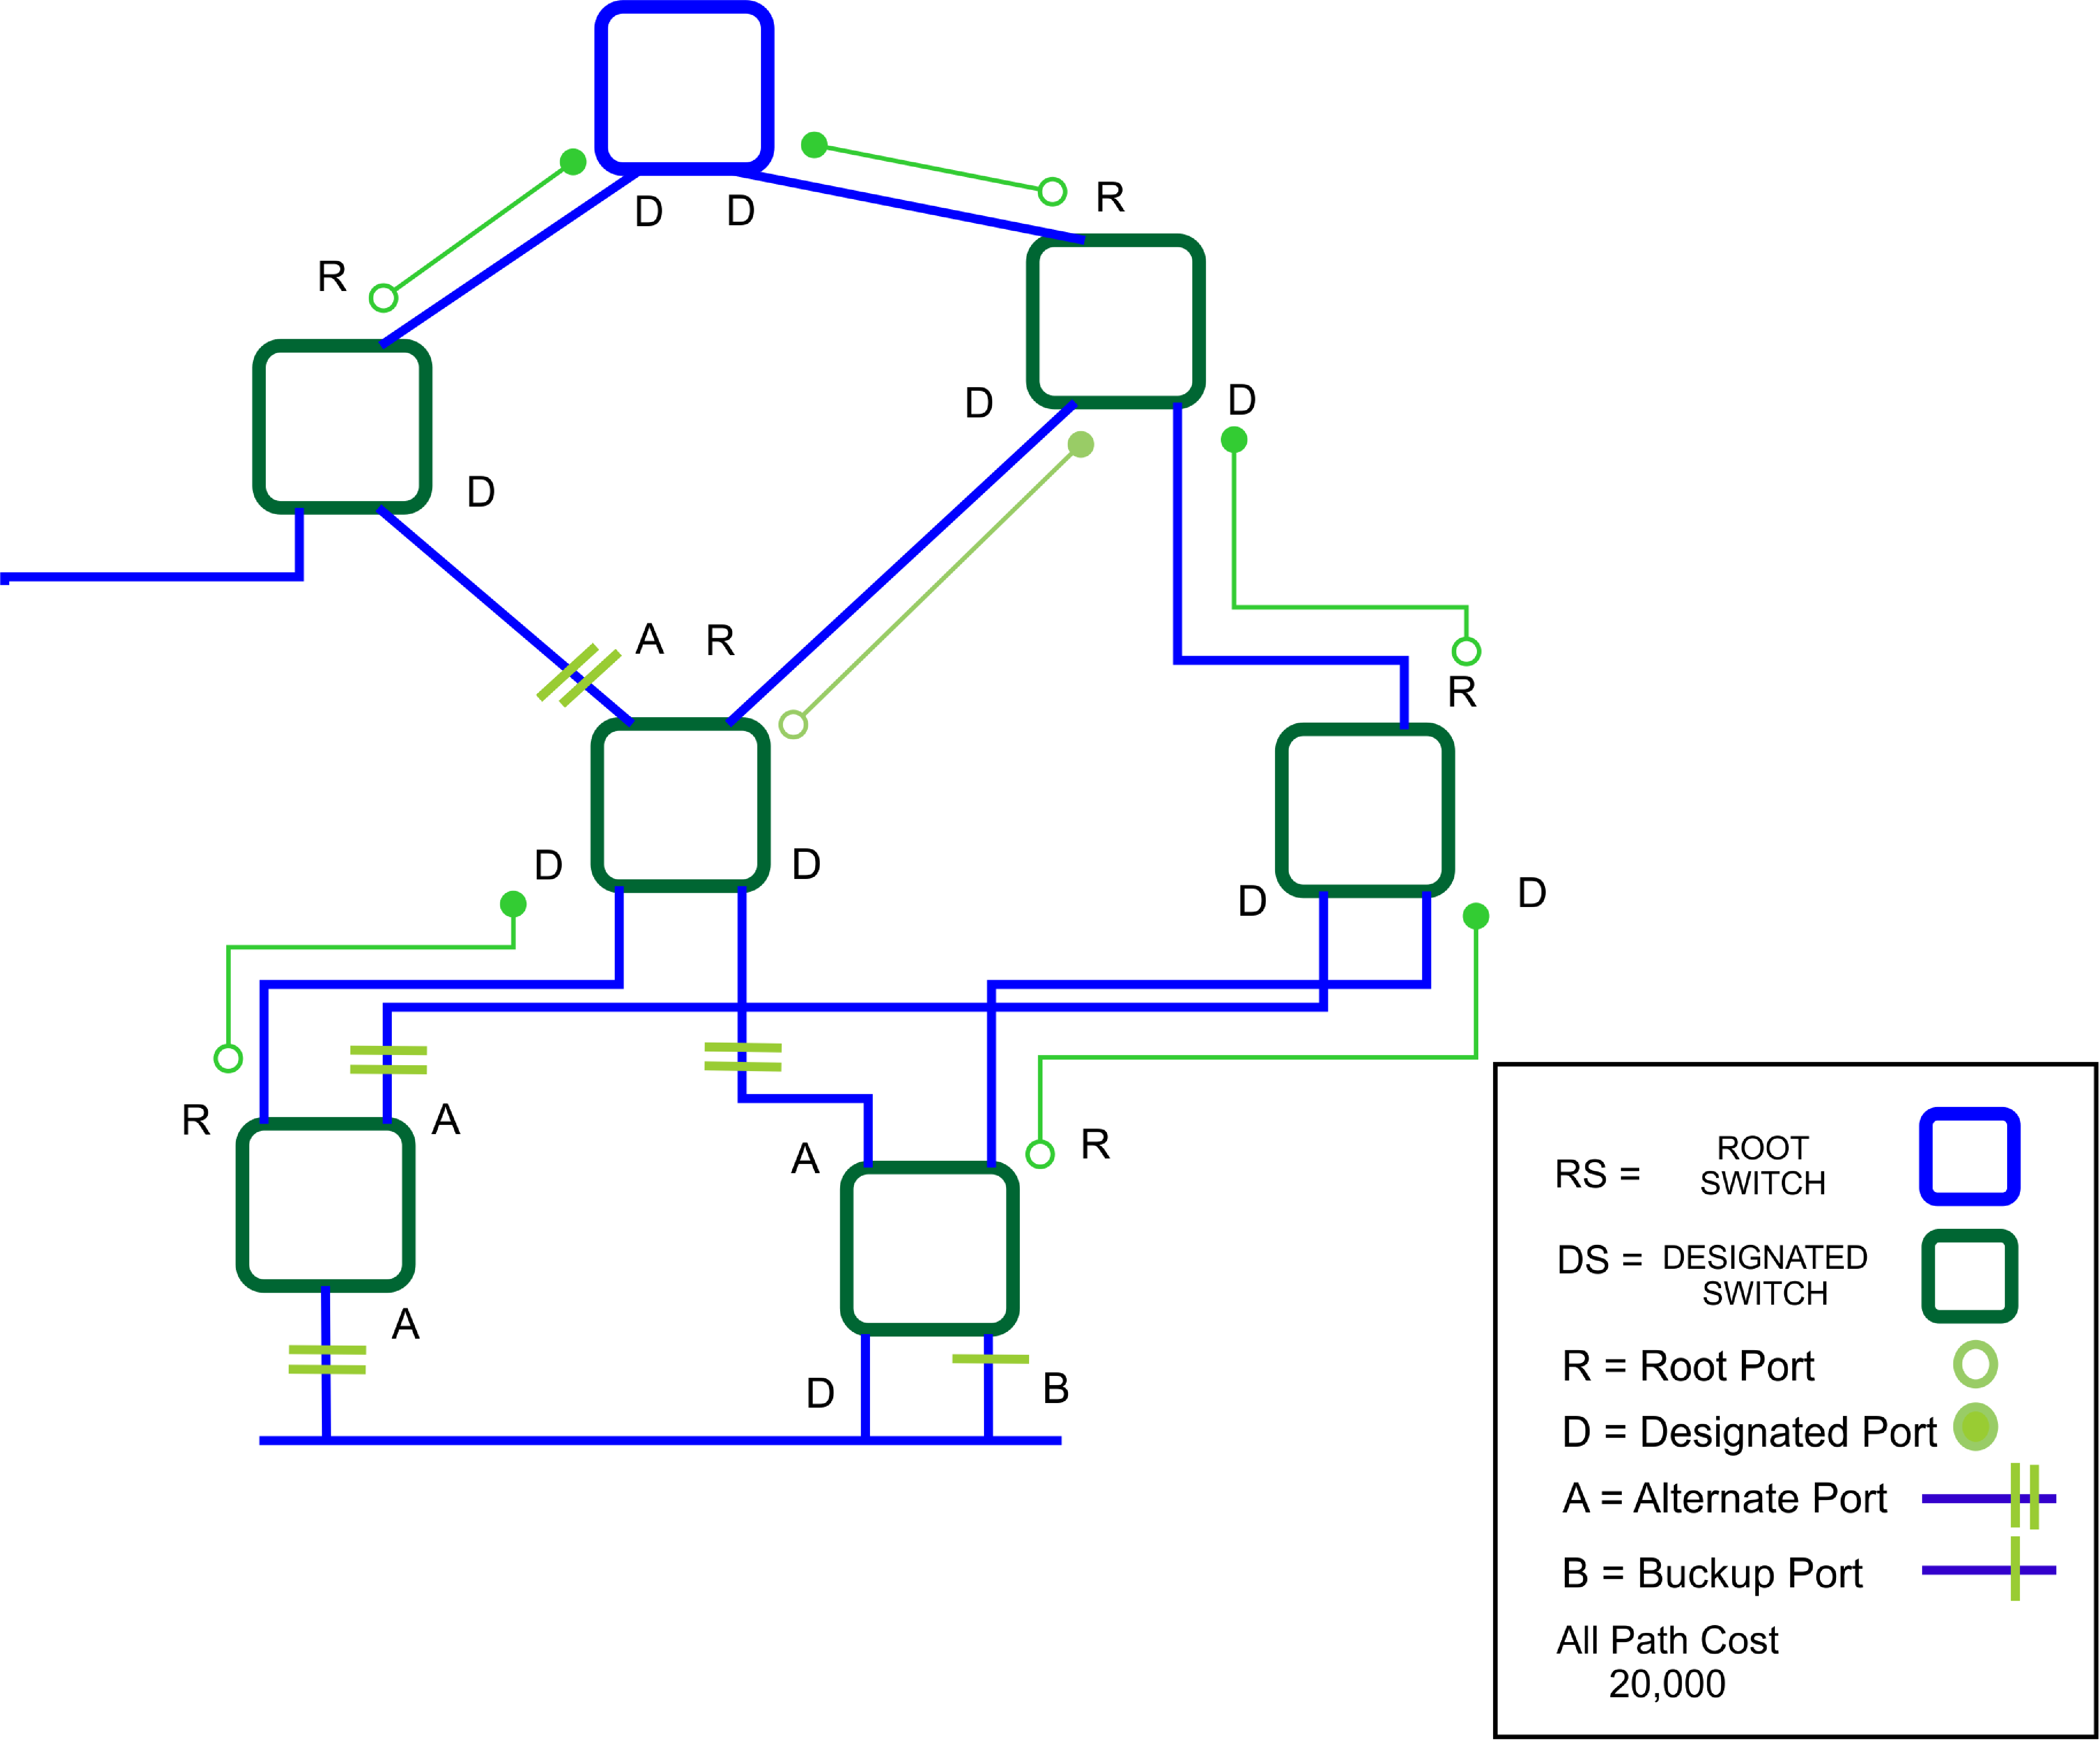
\includegraphics[scale=0.20 ]{robustness/network_spanning.pdf}
        \captionof{figure}{Free-Loops Network}
        \label{fig:free_loops}
\end{center}

The process of initial convergence it's not crucial for time
critical application, since it will be issued once the network is switched on.
Conversely, how ST deal with topologies changes and its
convergence, is extremely important for time critical application, like WR where
the packets tagged with the highest priority convey Control Information that
should not be lost due to a change of topology.

Normally, when a switch detects a topology change, it issues BDPU packets with
the Topology Change bit set. Every bridge that receives a BPDU with TC flag set,
should  receive it on either root port (coming from upstream) or designated port
(coming from downstream). The receiving bridge performs the following:
\begin{itemize}

        \item Flushes all MAC addresses associated with all ports with except to
the port where the TC BPDU was received
        \item Repeats the flooding procedure by starting Topology Change timer
and setting the TC bit for all BPDUs sent upstream or downstream. The receiving
port is excluded from flooding, in order to ensure flooding procedure
termination.
\end{itemize}
and the convergence process stars for this topology change. 



The end goal of STP is to ensure that only one port of a switch is responsible 
for forwarding traffic from the direction of the Root Switch onto any given
link. In networks running STP, every bridge has a priority value associated with
it, according with this value, the switch with the lowest priority will become
the Root of the network.  This process is done by the exchange of BPDUs packets
(Bridge Protocol Data Units) between switches. The rest of the switches shall be
Designated Switched, which forwards packets from the LAN toward the root bridge,
and vice versa.

\begin{center}
        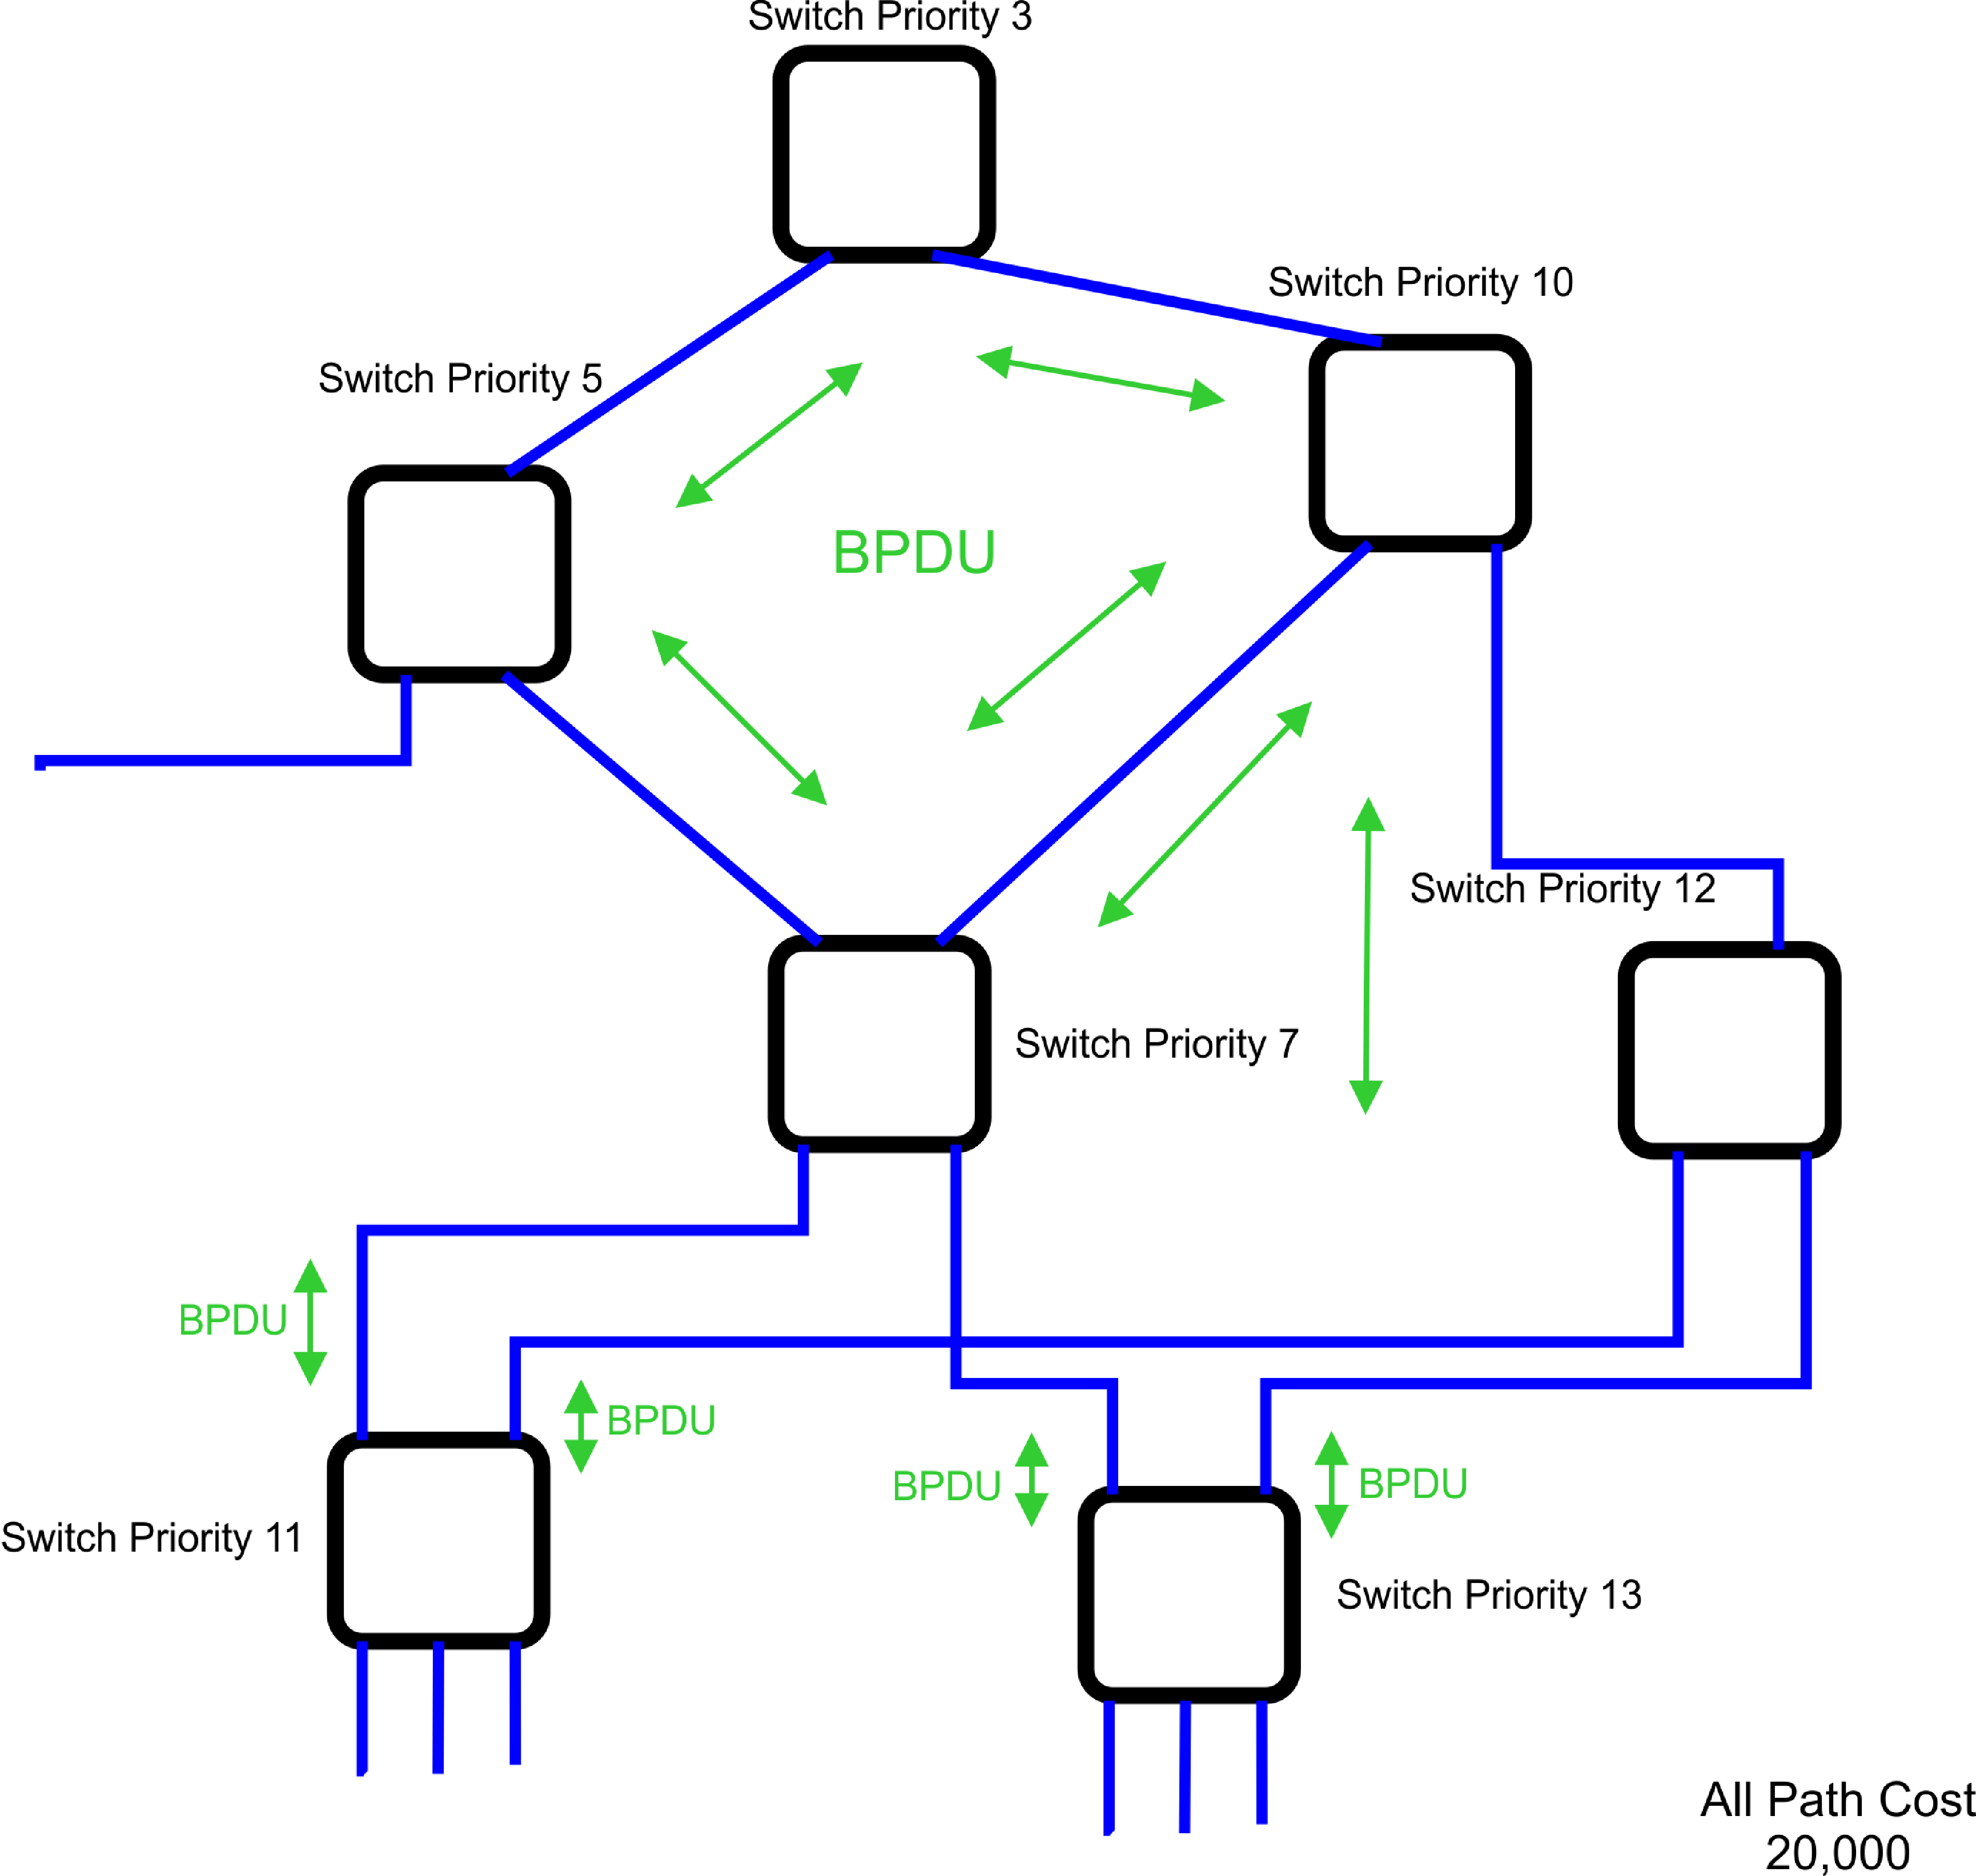
\includegraphics[scale=0.20 ]{robustness/network_beginning.pdf}
        \captionof{figure}{Redundant Network with Loops}
        \label{fig:redunt_net}
\end{center}


Once that the Root Switch has been defined, the switches shall determine
the least cost paths to the Root Switch. The cost is based on the number of
links from the switch till the root, and the cost of every link is based on the
Data Rate of the link. Data Rate ref(table of "Data rate and STP path cost"). In
case that two path have the same cost, there is a mechanism for breaking the
tie.

\begin{itemize}
        \item Root Port: provides connectivity to the root bridge
        \item Designated Port: forwards traffic from the root port onto the
next link.
        \item Alternate Port: an alternate path to the root bridge.
        \item Backup Port: a backup/redundant link to a segment where
another bridge port already connects.
\end{itemize}


RSTP implements distributed variation of Bellman-Ford iterative
algorithm, which could be described as "gradient" process, meaning it iteratively looks for the
optimal solution, selecting an "optimal" candidate every time. Every switch
(with except to the root) send and  accepts BPDU packets
with its information. The switch retains only the best current Root Switch
information electing one root port upstream toward the root switch. The switch
then block alternate paths to the root switch, leaving only the single optimal
upstream path and continue relaying optimal information downstream. If a switch
learns of a better root switch, on any of its ports, the previous "best"
information is erased and the new one immediately accepted and relayed. This
process will be propagated to all the switches, and it leads to the convergence
of the network where only one switch will be identified as root, and the rest of
the switches as designated with one port as Root Port and the rest designated,
Alternate or Backup Port.


\begin{center}
        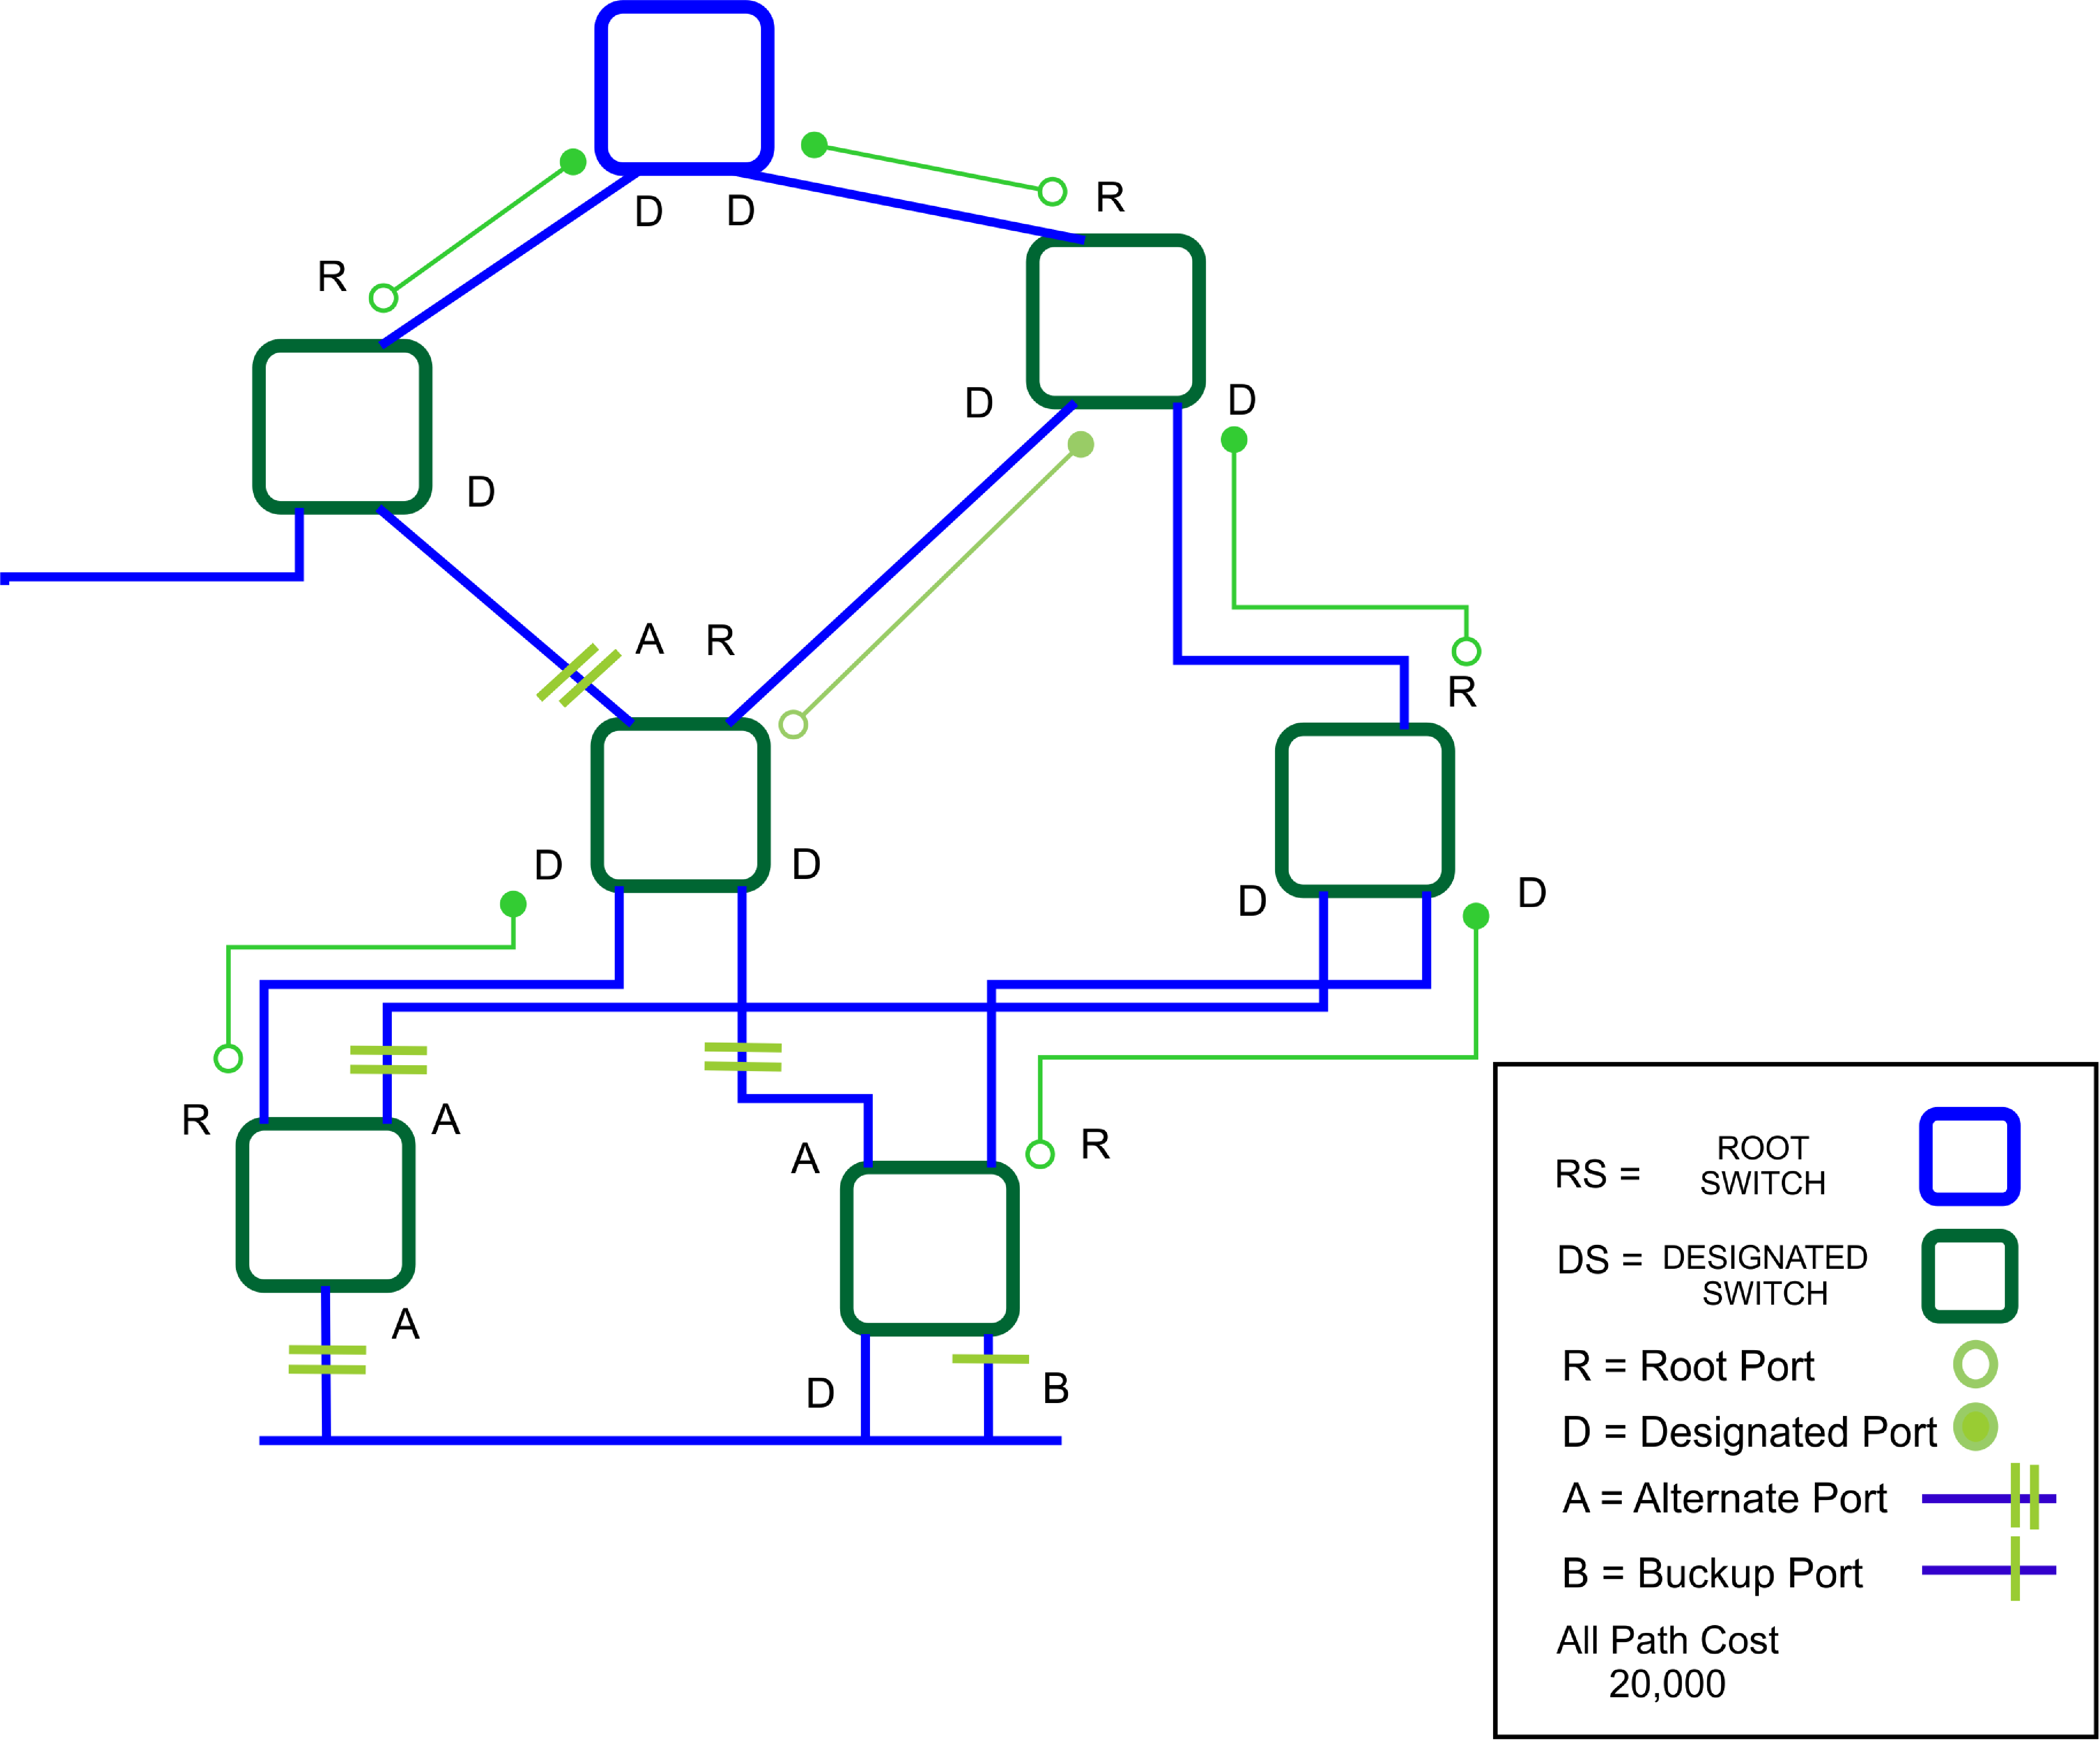
\includegraphics[scale=0.20 ]{robustness/network_spanning.pdf}
        \captionof{figure}{Free-Loops Network}
        \label{fig:free_loops}
\end{center}

The process of initial convergence it's not crucial for time
critical application, since it will be issued once the network is switched on.
Conversely, how ST deal with topologies changes and its
convergence, is extremely important for time critical application, like WR where
the packets tagged with the highest priority convey Control Information that
should not be lost due to a change of topology.

Normally, when a switch detects a topology change, it issues BDPU packets with
the Topology Change bit set. Every bridge that receives a BPDU with TC flag set,
should  receive it on either root port (coming from upstream) or designated port
(coming from downstream). The receiving bridge performs the following:
\begin{itemize}

        \item Flushes all MAC addresses associated with all ports with except to
the port where the TC BPDU was received
        \item Repeats the flooding procedure by starting Topology Change timer
and setting the TC bit for all BPDUs sent upstream or downstream. The receiving
port is excluded from flooding, in order to ensure flooding procedure
termination.
\end{itemize}
and the convergence process stars for this topology change. 

\subsection{Convergence in RSTP}

When a RSTP bridge detects a topology change by missing same BPDU seconds
(\textsl{Max Age Message}). Depending on the port state, the protocol will
handle the failure differently: 

\begin{itemize}

	\item If the port was blocking, nothing happens with except to expiring 
information associated with the failed port.
	\item If the port was designated, does nothing. However, downstream
switch may detect the loss of a root port and start converging. 
	\item If the port was a root: 

	\begin{itemize}
		\item It starts the  timer with a value equal to twice the 
hello-time (ref) for all its designated ports and its root port, if necessary.
		\item It flushes the MAC addresses associated with all these
ports.
	\end{itemize}

\end{itemize}


When a switch receives a BPDU with the TC bit set from a neighbor:

\begin{itemize}
 
	\item It clears the MAC addresses learned on all its ports, except the 
one that receives the topology change. 
	\item It starts the timer and sends BPDUs with Topoloy Change set on all
 its designated ports and root port.
\end{itemize}

This way, the Topology Change Notification floods very quickly across the whole 
network. The Topology Change propagation is now a one step process. In fact, the
initiator of the topology change floods this information throughout the network.

In just a few seconds, or a small multiple of hello-times, most of the entries 
in the routing tables of the entire network flush. This approach results in
potentially more temporary flooding, but on the other hand it clears potential
stale information that prevents rapid connectivity restitution. 



\textbf{Convergence in Dual Link Topology}

The Dual Link Topology a particular case of fast recovery. Both switches detects
 failure of a link  simultaneously and immediately age out the learned MAC
address entries for these ports. Bridge B has been receiving periodic
transmissions of BPDUs on the other link. This information allows it to evaluate
the second link as its best path to the to the root bridge. Bridge B immediately
sets its root port. 

RSTP procedure requires a topology change when adding a path to the topology. 
Bridge B "sees" the new root port as an added path and floods topology changes
out its ports. Though not strictly necessary in this case, they cause no ill
effects.

\begin{center}
        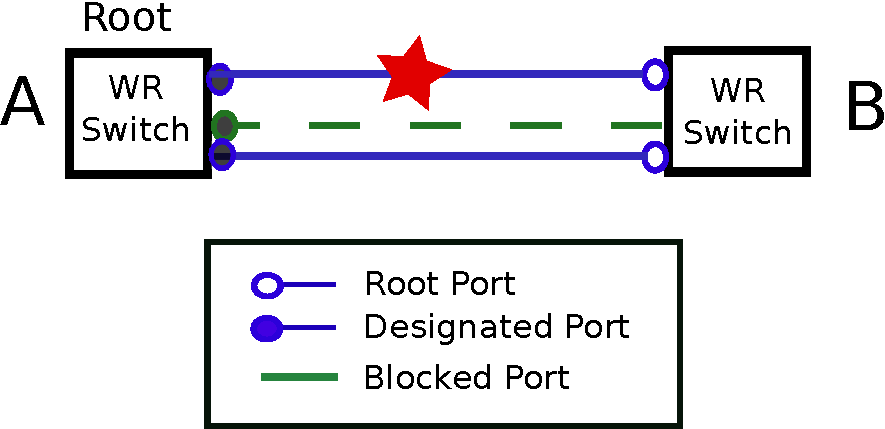
\includegraphics[scale=0.70 ]{robustness/dual_link.pdf}
        \captionof{figure}{Convergence Dual Link Topology}
        \label{fig:idual_link}
\end{center}

\textbf{Convergence in case of Root Port Loss}

The switch C  detects loss of the root port, by missing BPDUs for same time 
(e.g. 3xHello time). Next, the following is the sequence of events that occurs:

The switch C declares loss of the root bridge. Since the switch has no other 
paths to the root, it declares
itself as the new root bridge for the topology and attempts to synchronize  this
information with the rest of 
the topology. The synchronization wave will propagate through Switch B and 
eventually reaches D, which has better root port information. The sync wave
bounces back and goes till C to adapt to the new information and will declare
the designated port as root port.

\begin{center}
        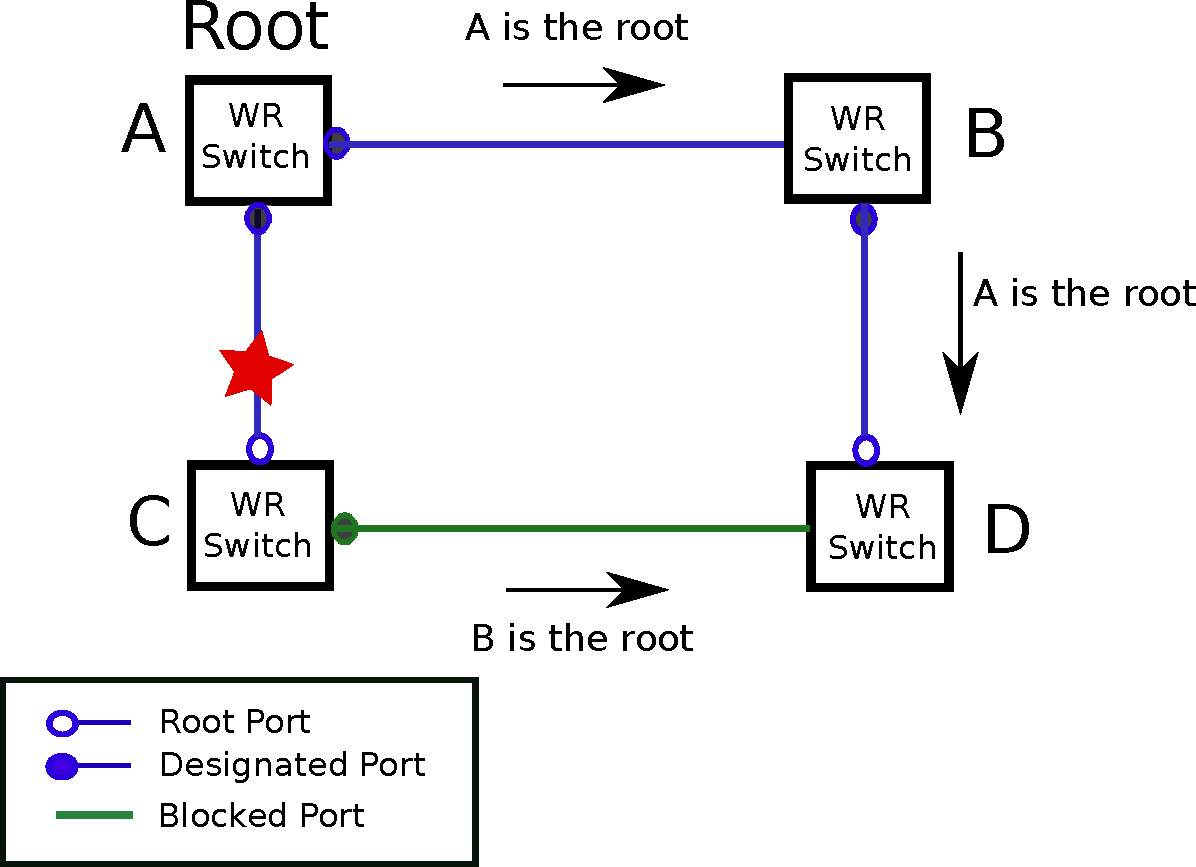
\includegraphics[scale=0.70 ]{robustness/indirect_change_explamation.pdf}
        \captionof{figure}{Convergence Indirect Change of Topology}
        \label{fig:indirect_change}
\end{center}

\section{White Rabbit RSTP Use Cases}

\begin{center}
	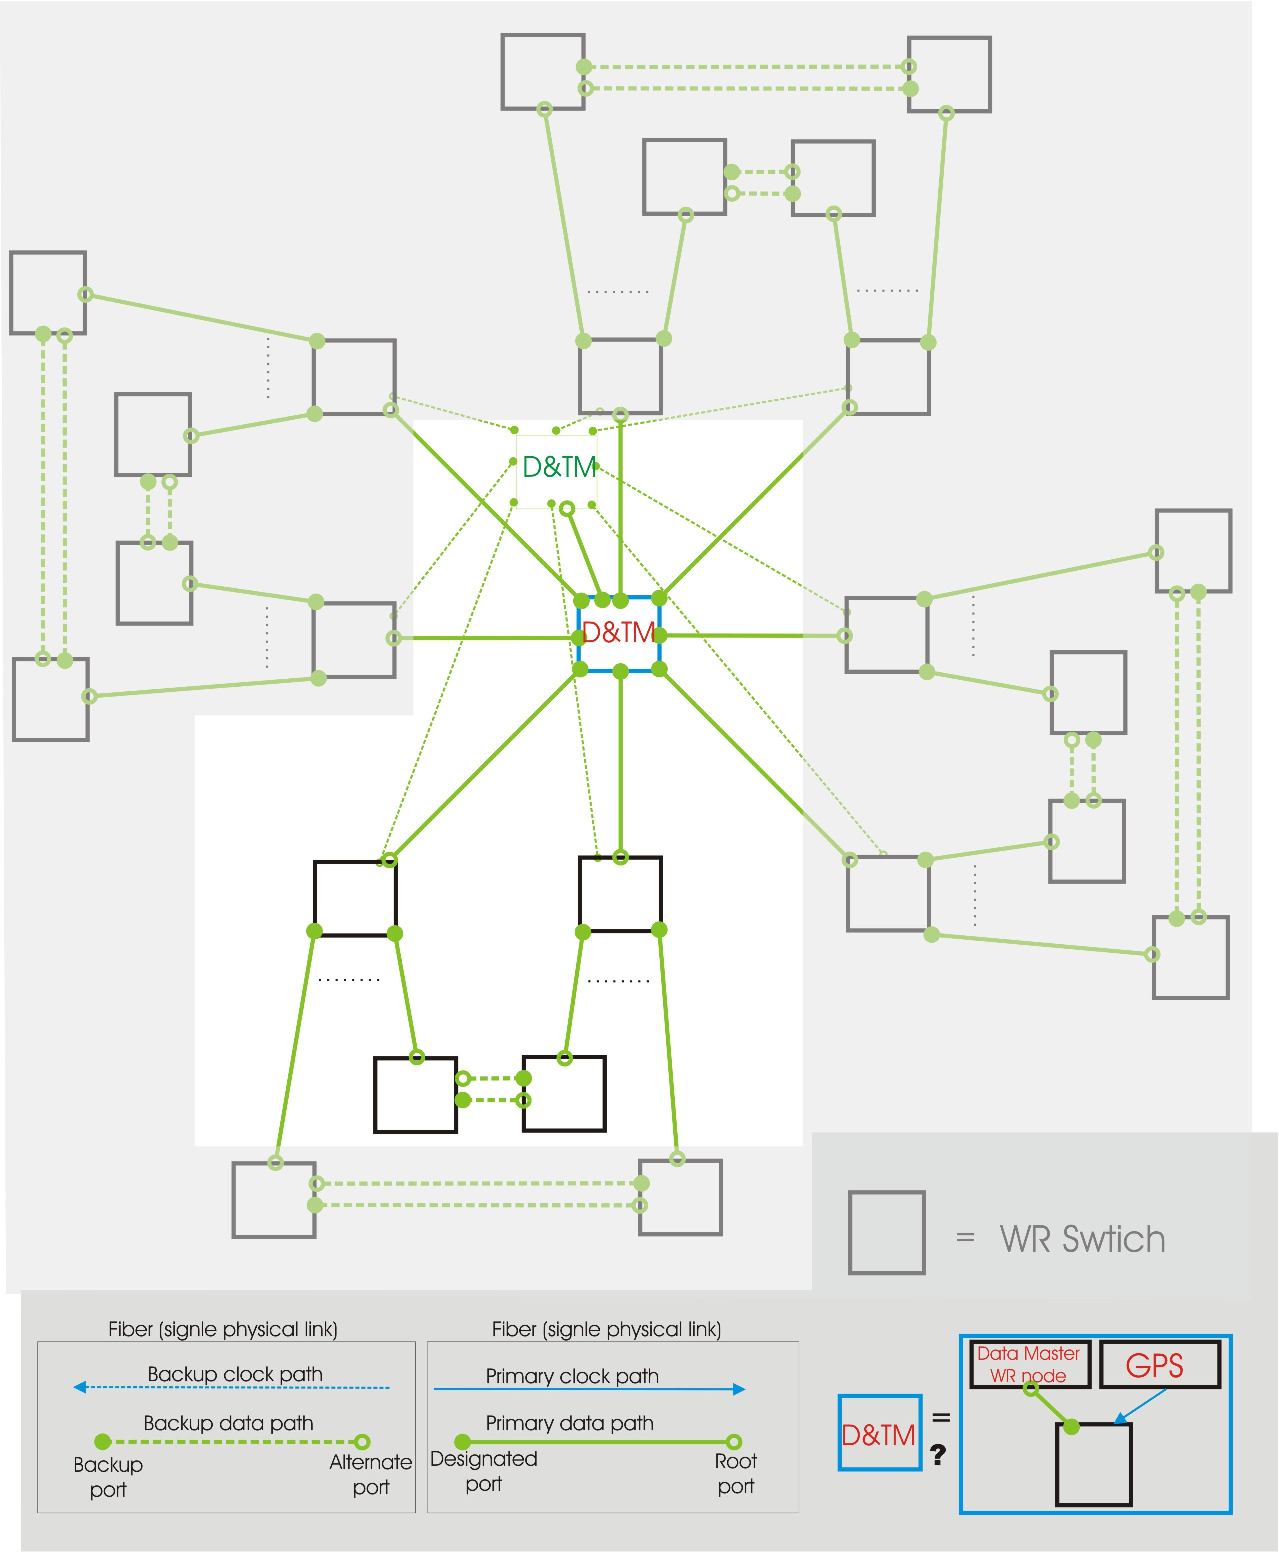
\includegraphics[scale=0.40]{robustness/WRRSTPforHP.pdf}
	\captionof{figure}{Some topology of the network and the bit we are
considering.}
	\label{fig:WRRSTPforHP}
\end{center}

\begin{center}
	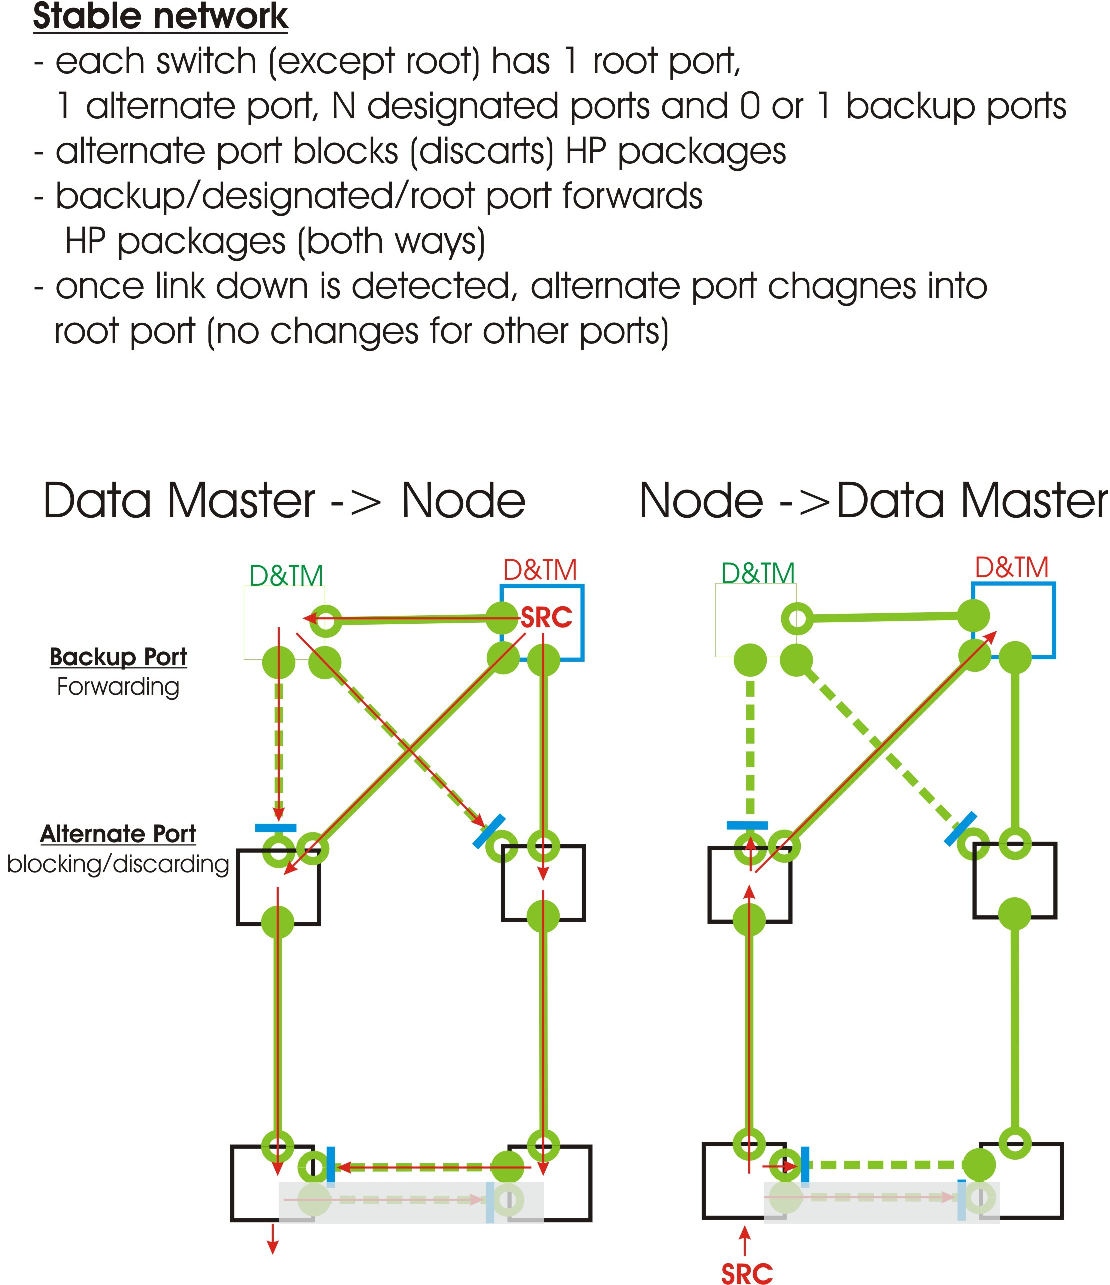
\includegraphics[scale=0.40]{robustness/WRRSTPforHP2.pdf}
	\captionof{figure}{The considered fragment of the network.}
	\label{fig:WRRSTPforHP2}
\end{center}

\begin{center}
	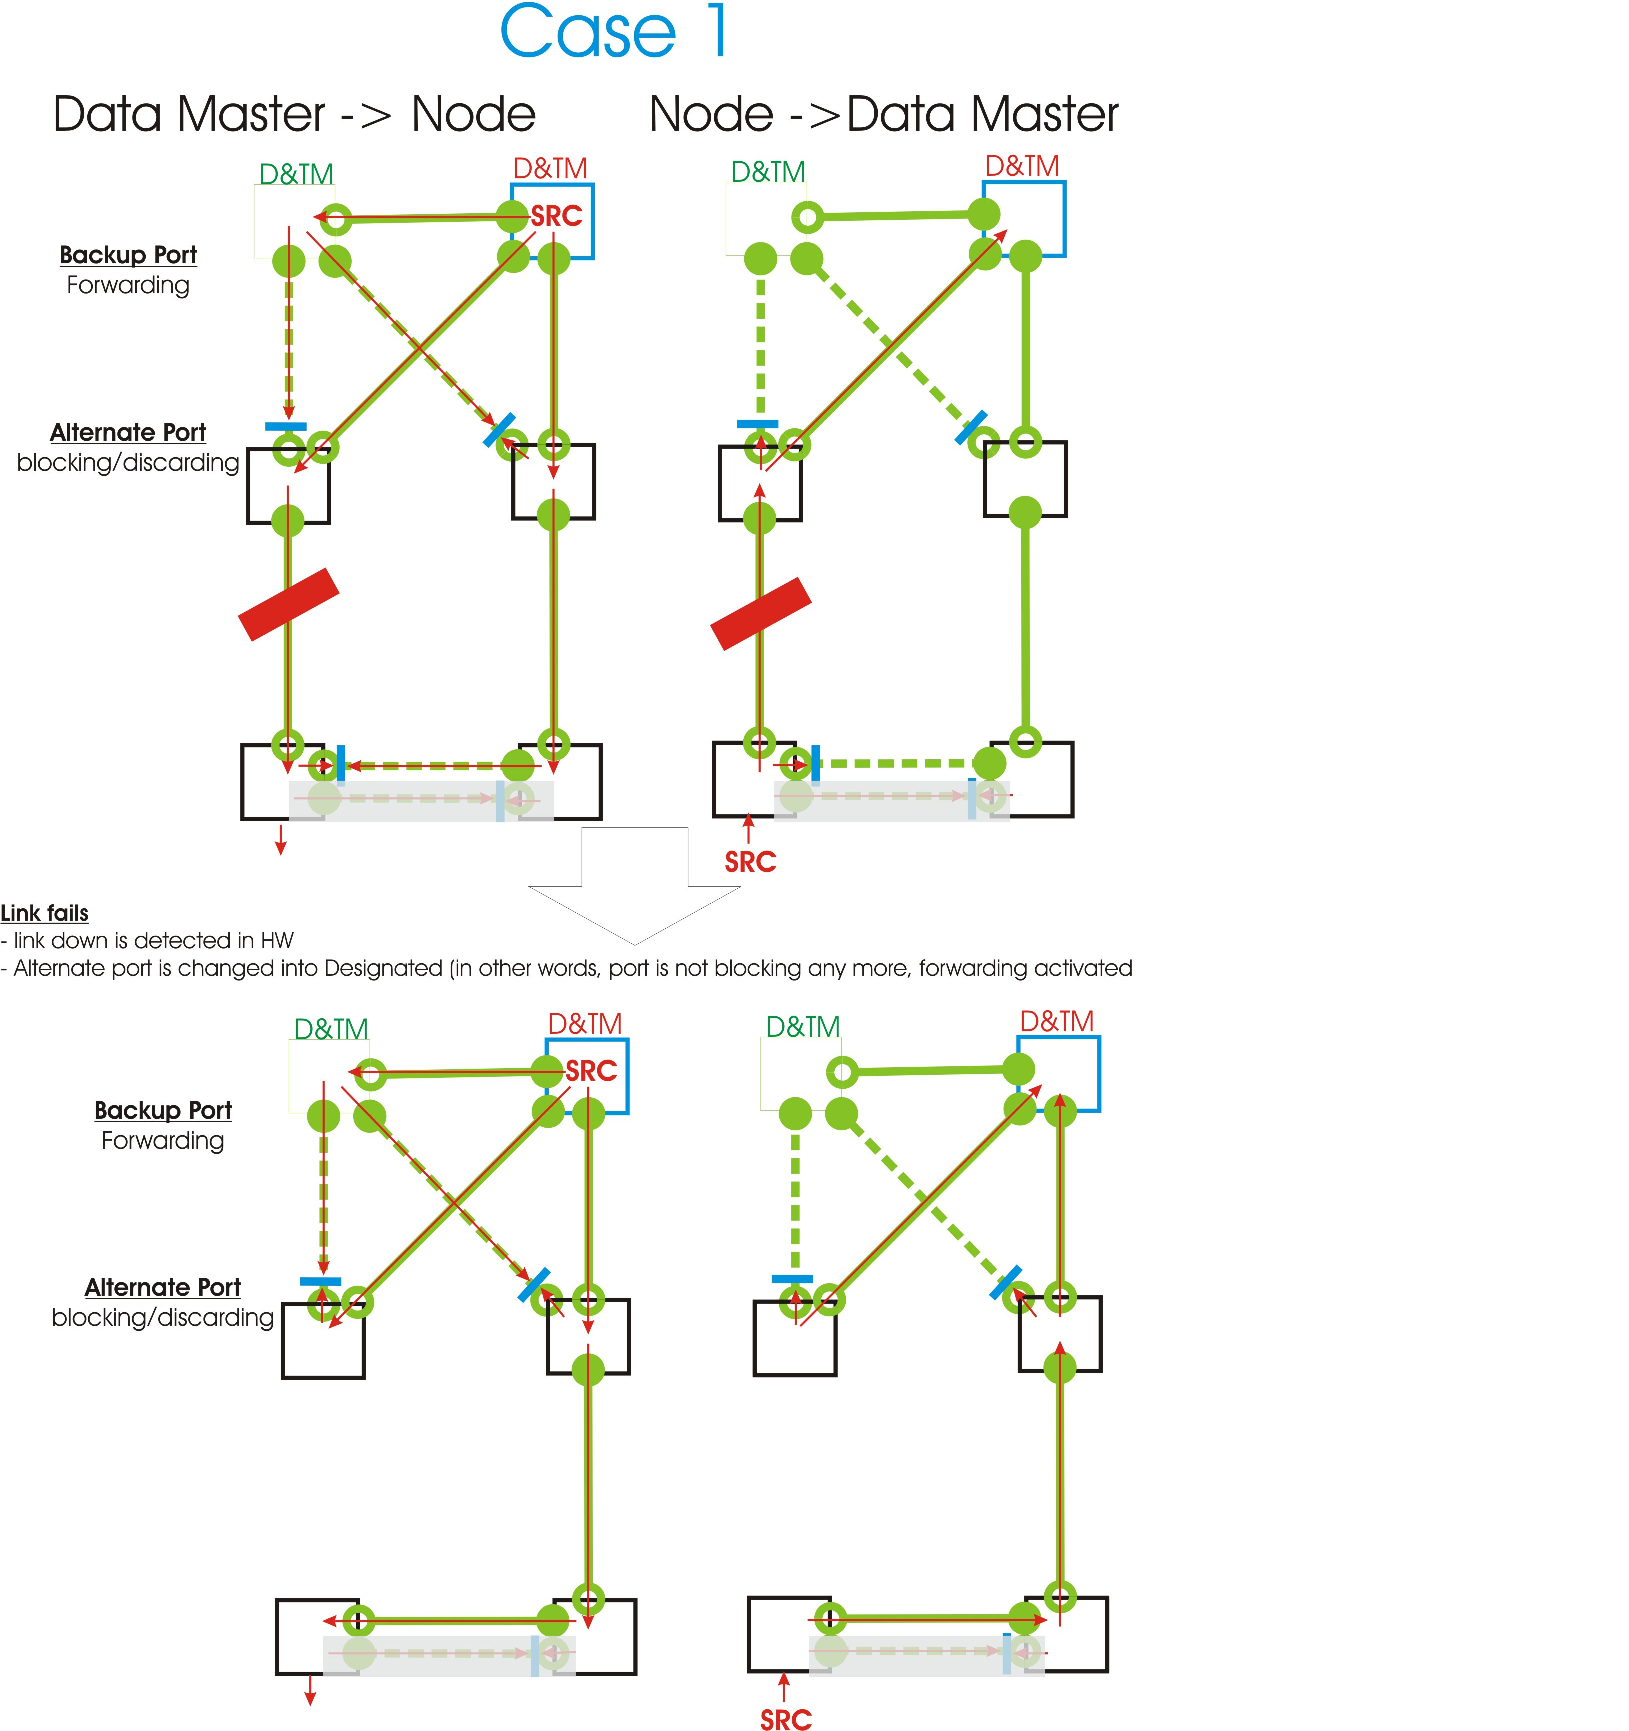
\includegraphics[scale=0.40]{robustness/WRRSTPcase1.pdf}
	\captionof{figure}{Link failure Use Case.}
	\label{fig:WRRSTPcase1}
\end{center}

\begin{center}
	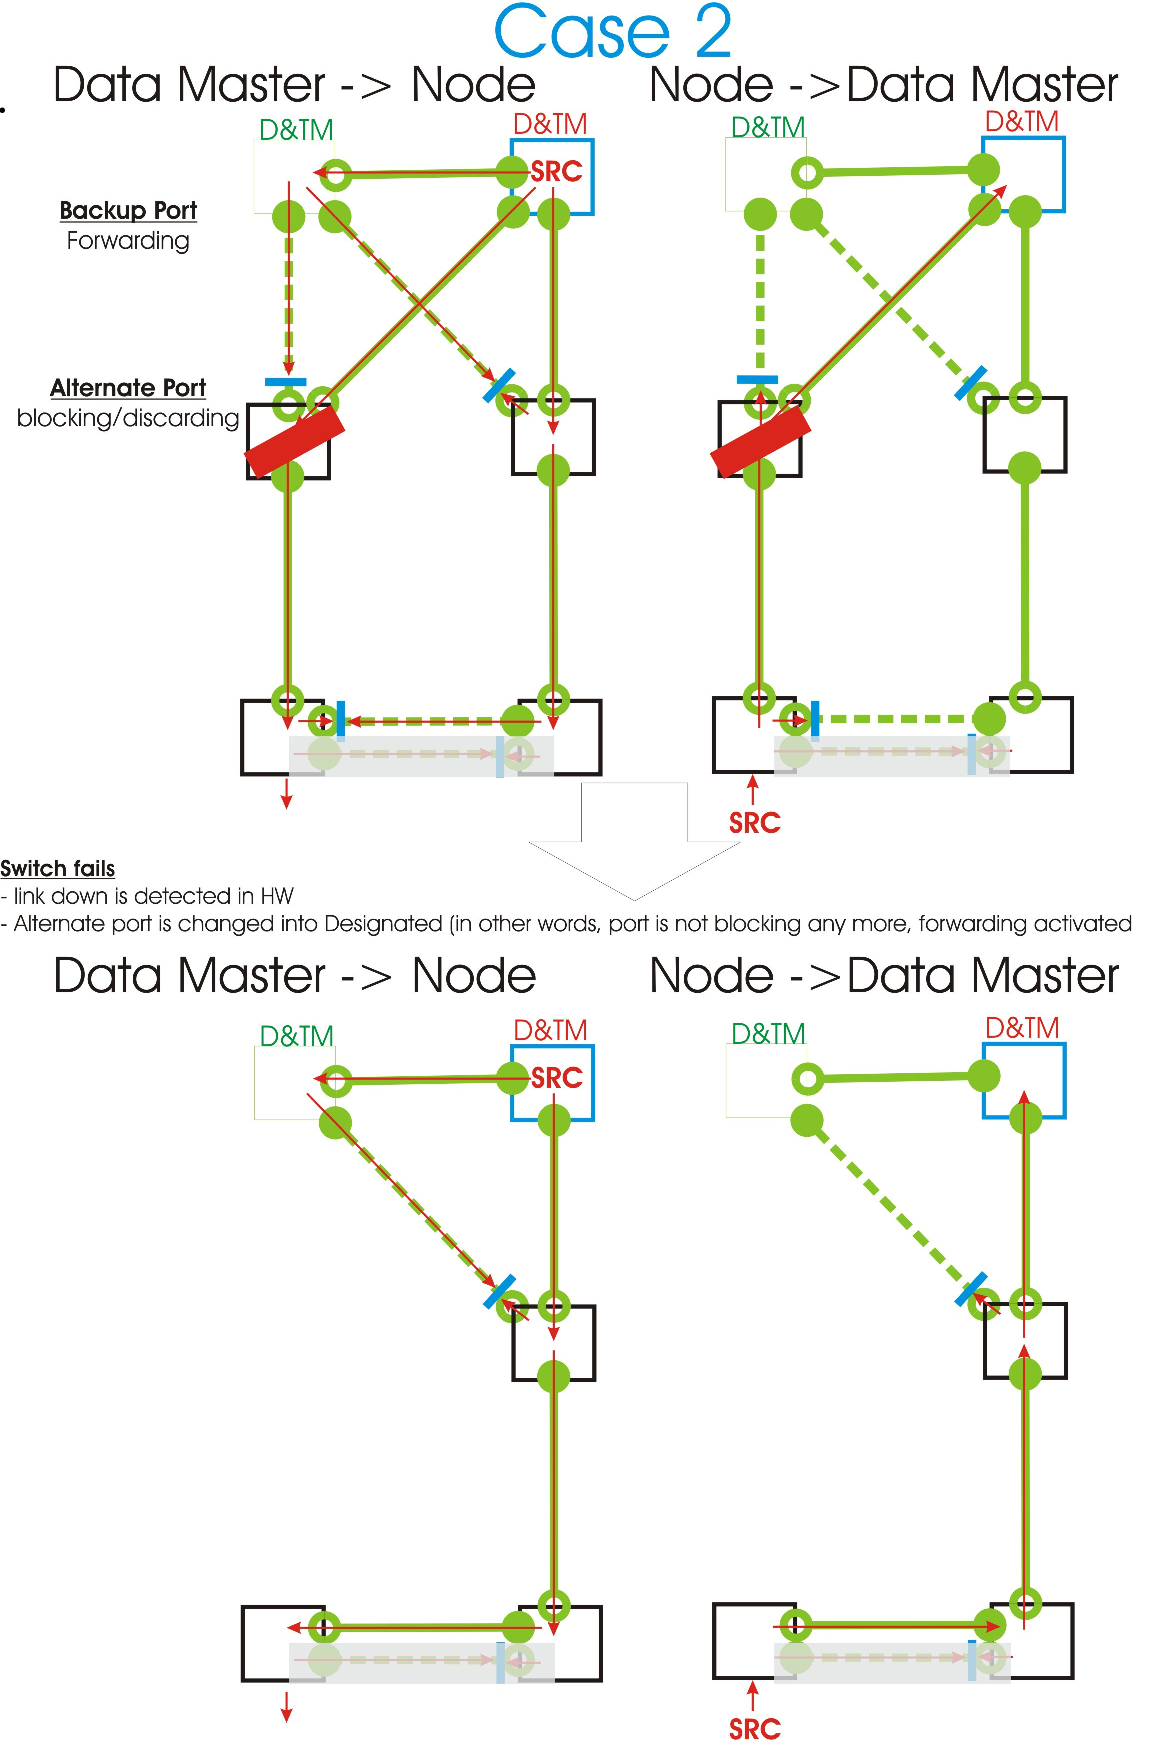
\includegraphics[scale=0.40]{robustness/WRRSTPcase2.pdf}
	\captionof{figure}{Switch failure Use Case.}
	\label{fig:WRRSTPcase2}
\end{center}
\begin{center}
	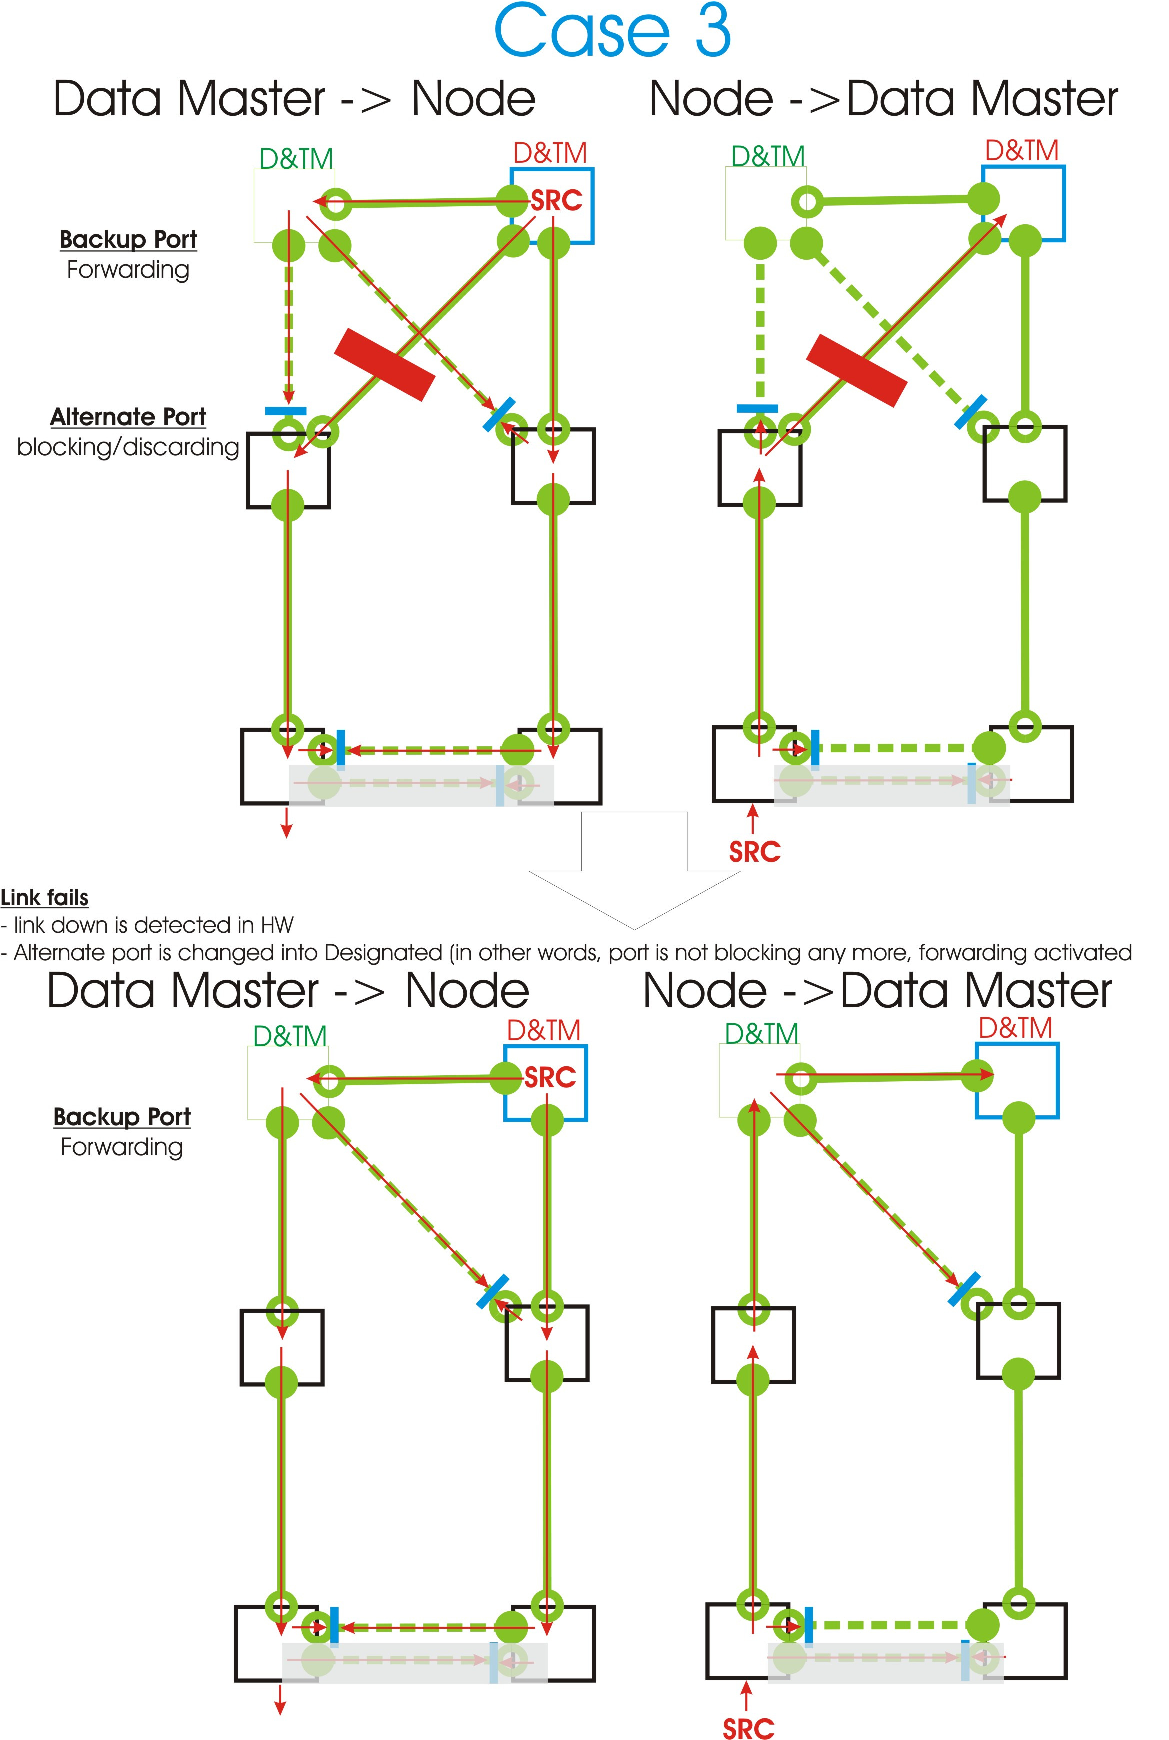
\includegraphics[scale=0.40]{robustness/WRRSTPcase3.pdf}
	\captionof{figure}{Link failure Use Case.}
	\label{fig:WRRSTPcase3}
\end{center}

\begin{center}
	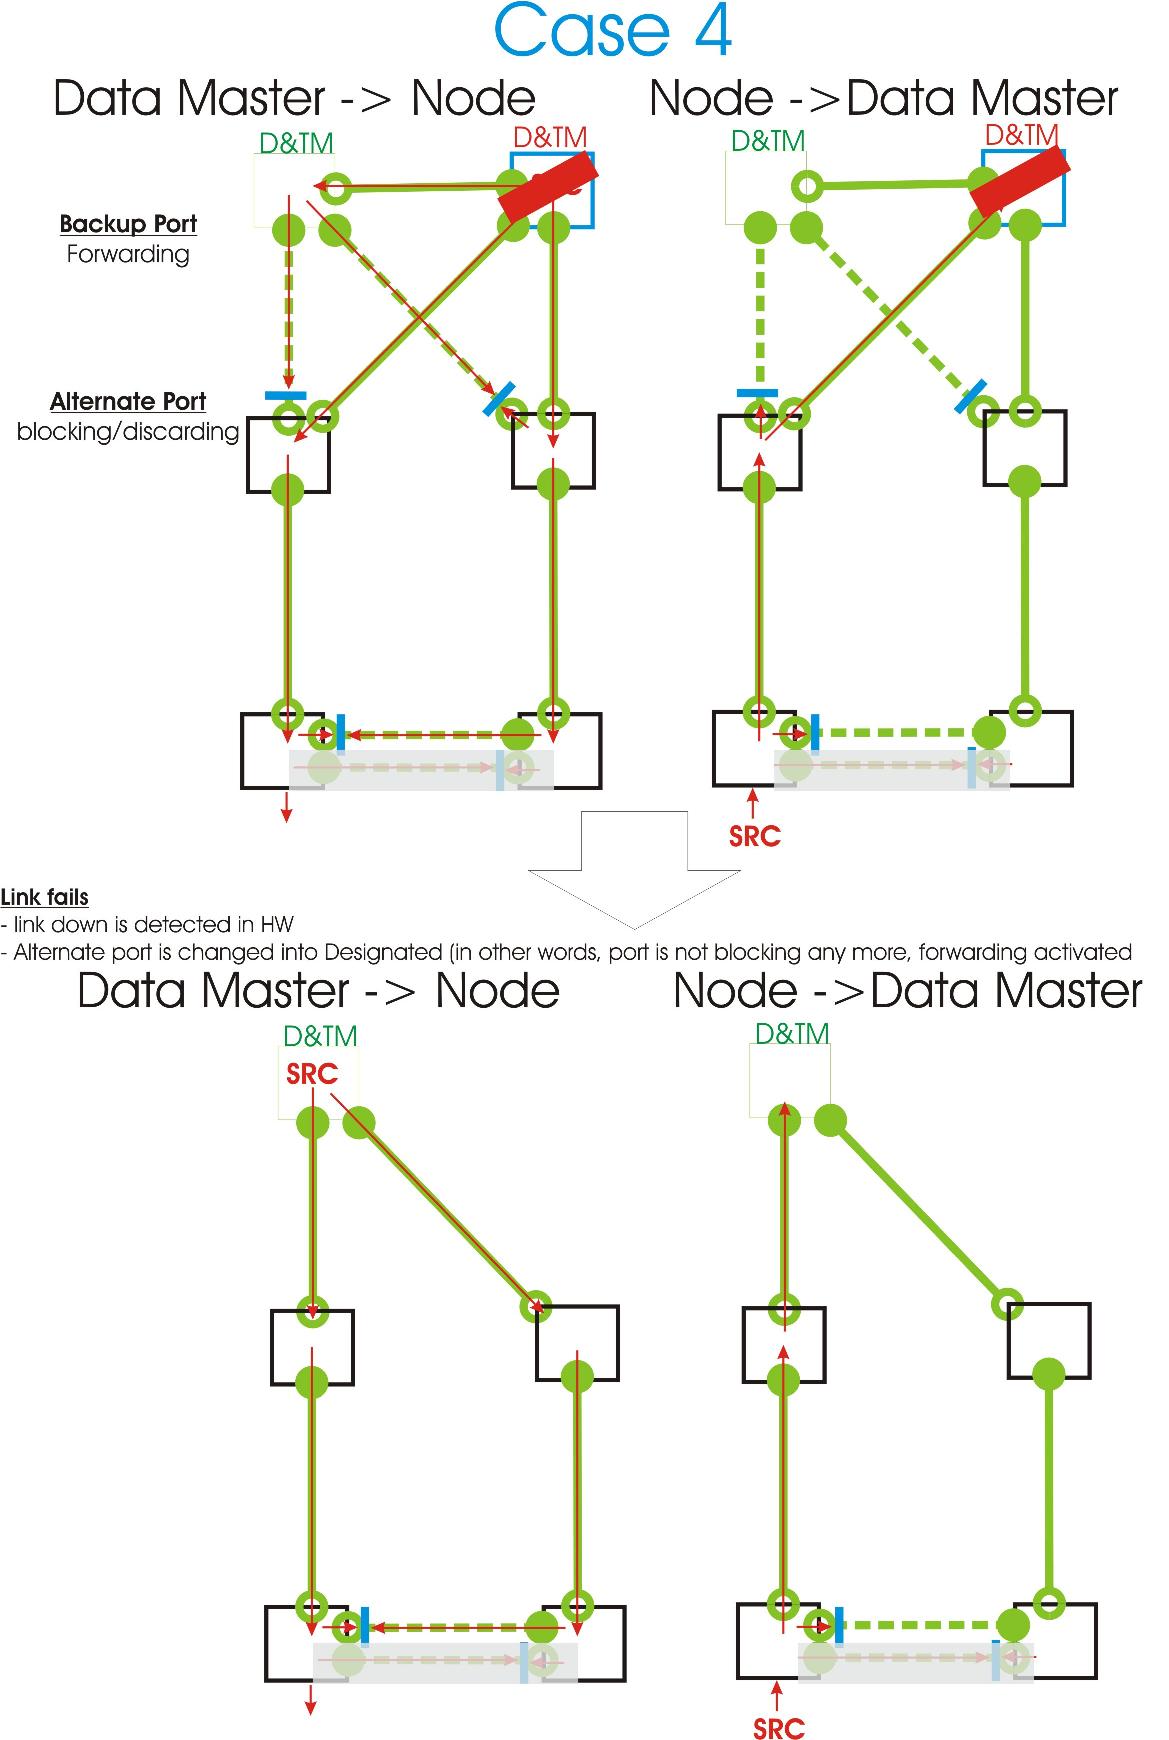
\includegraphics[scale=0.40]{robustness/WRRSTPcase4.pdf}
	\captionof{figure}{Failure of the switch connected to Data Master Node
(assuming flawless switching to backup Data Master.}
	\label{fig:WRRSTPcase4}
\end{center}

\begin{center}
	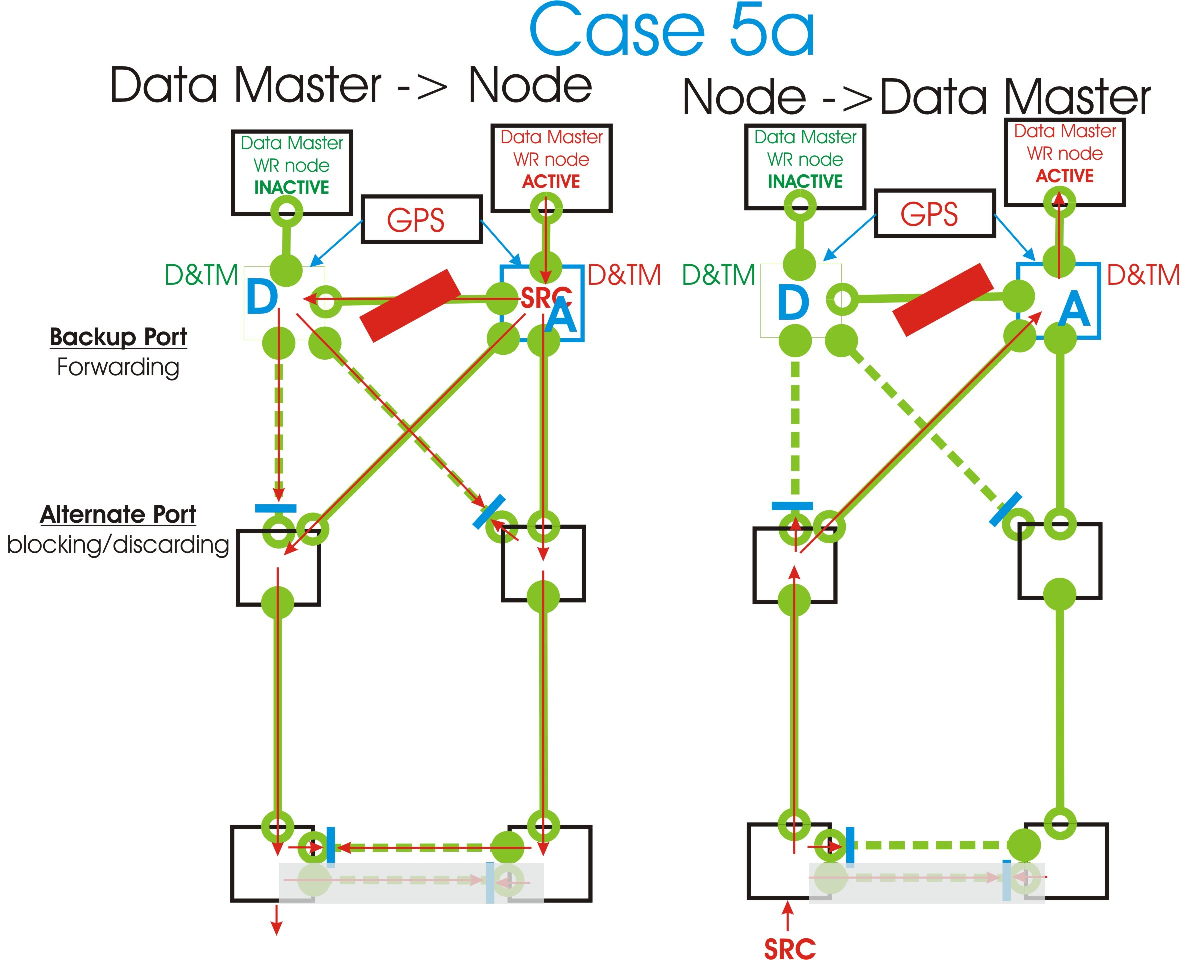
\includegraphics[scale=0.40]{robustness/WRRSTPcase5.pdf}
	\captionof{figure}{Link Failure between switches connected to
Master Node and backup Master Node}
	\label{fig:WRRSTPcase5}
\end{center}

\section{Solutions to overcome RSTP limitations}
The proposed solution has its limitation, to overcome this shortcomings, three
solutions are considered:
\begin{itemize}
  \item Map/Table of possible changes of topology in each
switch + WR BPDU, in HW (Non-Standard). 
  \item WR BPDU + using RSTP data + some additional logic, in HW (Non-standard,
).
  \item WR BPDU + using RSTP data + some additional logic, in HW
(Almost-standard).
\end{itemize}
They are not to be described in details in the first release of the document,
these are exceptional/rare cases.
